\documentclass[a4paper]{article}

\usepackage[english]{babel}
\usepackage[utf8]{inputenc}
\usepackage{amsmath}
\usepackage{graphicx}
\usepackage[colorinlistoftodos]{todonotes}
\usepackage{hyperref}
\usepackage{listings}
\usepackage[numbers]{natbib}

\usepackage{booktabs} % To thicken table lines



\title{Creating Customer Segments}

\author{Uirá Caiado}

\date{\today}

\begin{document}

\maketitle

\begin{abstract}
bla
\end{abstract}

%%%%%%%%%%%%%%%%%%%%%%%%%%%%%%%%%%%%%%%%%%%%%%%%%%%%%%%%%%%%%%%%%%%%%%%%%%%%%%%%%%%%%%%%
%% INTRODUCTION
%%%%%%%%%%%%%%%%%%%%%%%%%%%%%%%%%%%%%%%%%%%%%%%%%%%%%%%%%%%%%%%%%%%%%%%%%%%%%%%%%%%%%%%%

\section{Introduction}
\label{sec:introduction}

\subsection{Bla}
As stated by Udacity\footnote{Source: \url{https://goo.gl/i8TQwZ}}  and bla.

Bla bla bla.

\subsection{The Goal}
bla bla bla

\subsection{Bla}
Bla and \cite{Hastie_2009}, tbla bla bla.

%%%%%%%%%%%%%%%%%%%%%%%%%%%%%%%%%%%%%%%%%%%%%%%%%%%%%%%%%%%%%%%%%%%%%%%%%%%%%%%%%%%%%%%%
%% EXPLORING THE DATA
%%%%%%%%%%%%%%%%%%%%%%%%%%%%%%%%%%%%%%%%%%%%%%%%%%%%%%%%%%%%%%%%%%%%%%%%%%%%%%%%%%%%%%%%


\section{Exploring the Data}
\label{sec:exploring_data}
In this section, we will explore the data to look for insides about the features.

\subsection{Basic Facts}
Let's go ahead and execute a basic description of the student dataset (Table \ref{tab:basicfacts}):

\begin{table}[ht]
\centering
\begin{tabular}{l|r}
 & Value \\\hline
Total number of students & 42 \\
Total number of students & 395 \\
Number of students who passed & 265 \\
Number of students who failed & 130 \\
Number of features & 30 \\
Graduation rate of the class & 67.09 \%

\end{tabular}
\caption{\label{tab:basicfacts}Facts About the Dataset.}
\end{table}

Bla

\subsection{Bla}
bla bla.

\begin{figure}[ht]
\centering
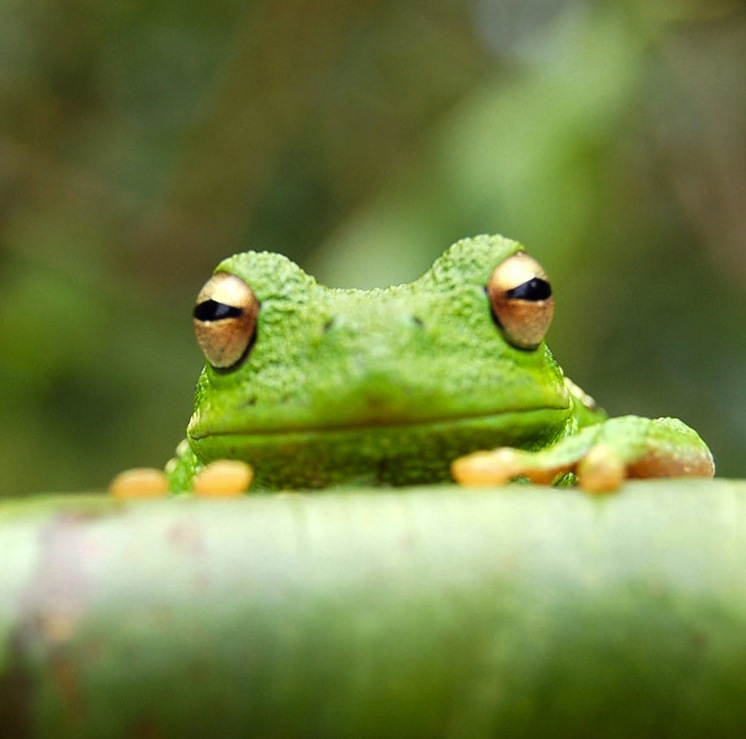
\includegraphics[width=0.45\textwidth]{figures/frog.jpg}
\caption{\label{fig:categorical}Categorical Data.}
\end{figure}

bla

%%%%%%%%%%%%%%%%%%%%%%%%%%%%%%%%%%%%%%%%%%%%%%%%%%%%%%%%%%%%%%%%%%%%%%%%%%%%%%%%%%%%%%%%
%% REFLECTION
%%%%%%%%%%%%%%%%%%%%%%%%%%%%%%%%%%%%%%%%%%%%%%%%%%%%%%%%%%%%%%%%%%%%%%%%%%%%%%%%%%%%%%%%

\section{Reflection}
Bla bla bla




\bibliographystyle{plain}
% or try abbrvnat or unsrtnat
\bibliography{bibliography/biblio.bib}
\end{document}